
\newcommand{\Freg}{\( F_{reg} \)}


\section*{Abstract}
\textbf{Genetics has been a cornerstone of biology since its inception almost
100 years ago. However, the rules of genetic inference remain
axiomatic, and as a result, confusion regarding these rules abounds. Here, I
show that Batesonian epistasis, which has been used to construct genetic
networks, emerges naturally from a statistical mechanical framework. I will show
how the inferences of genetic interactions on the basis of Batesonian epistasis
emerge from this framework, thus establishing that the methods geneticists use
to identify interactions amongst genes can be viewed as a non-analytical
variational method to probe an unknown partition function. By establishing
Batesonian epistasis, this method can constrain the properties of this unknown
partition function and reveal how variables within this partition function are
functionally related to each other.
}

\section*{Introduction}
Biological processes can be broadly subdivided into two large categories:
Processes where the players and interactions are known, and processes where the
players or the interactions are unknown. Necessarily, the study of processes in
either category varies substantially, as do the available methodologies.
Processes where the components are unknown cannot be studied in a predictive
fashion and mathematical methods cannot be used to identify the components that
participate in the process (though they can make statements about the properties
these components must exhibit). On the other hand, when the major components and
interactions of a system are known, detailed models can be built to study
emergent properties present in the system or to identify the regimes in which
the model breaks down, thus indicating missing information about the system.

A particularly effective method for modeling a large number of physical
phenomena is statistical mechanics. Statistical mechanics dictates that if all
the possible configurations of a system are known (all the states and their
weights), then the probability that an event happens is equal to the weighted
sum of the states that can lead to that event divided by the weighted sum of all
the possible states. The weighted sum of all the possible states is particularly
important and is called the Partition Function. Though this theory was
originally applied to ideal gases, it has become widespread, finding
applications in all areas of physics, but also in biology~\citep{Garcia2007},
neurobiology~\citep{Schneidman2006} and even the social
sciences~\citep{Lee2015}. Statistical mechanical models demand a detailed and
quantitative knowledge of the system to be tractable.

In contrast to the quantitative description of a physical phenomenon obtained
from statistical mechanical models, genetics is a favored approach when the
system is completely unknown, because the genetical framework is explicitly
designed to make as few assumptions as possible. Saturating genetic screens can
be used to find all of the genes that cause a specific phenotype when
mutated~\citep{Brenner1974,Jurgens1984}. Once these genes are known, epistatic
analyses using null mutants of these genes can establish genetic interactions
between these genes.

Genetic interactions describe the broadest possible mode of interaction in a
biological system. Formally, two genes genetically interact if they affect the
same phenotype. However, not all gene interactions are considered equally
informative; the set of uninformative genetic interactions are defined by the
choice of null hypothesis, which is often selected to be a multiplicative null
hypothesis (also known as log-additive null hypothesis). A more strict and
informative definition of genetic interactions requires:

\begin{enumerate}
  \item The two genes control the same phenotype;
  \item The phenotype of the double null mutant deviates from that expected
  under a null model of interaction
\end{enumerate}

The deviation between the expected phenotype and the observed phenotype of the
double mutant is an important quantity that we refer to as generalized
epistasis~\citep{Fisher1919}. Although generalized epistasis can take on any
value in theory, in the context of developmental genetics, generalized epistasis
measured between two genes using null mutants often reduces to a limited set of
specific values. These values correspond to a phenomenon we refer to as complete
epistasis, which is important for classical developmental genetics. Complete
epistasis refers to a situation where the double mutant exhibits exactly the
same phenotype as one of the single mutants, originally defined by
Bateson~\citep{Bateson2009}. Measuring this equality is equivalent to
constraining the value of the generalized epistasis term to a unique value.
The relationship between classical and generalized epistasis has been a source
of great confusion, not least because multiple fields use conflicting
definitions for the term and use it to measure different
things~\citep{Cordell2002,Phillips2008}. A major problem is that the presence of
generalized epistasis depends strongly on the choice of null model. In this
text, we only use the term epistasis, either complete or generalized, to refer
to the situation where the double mutant exhibits the same phenotype as one of
the corresponding single mutants. We will use the word `mutant' to refer to a
null allele, unless otherwise specified. Finally, we will use the term
`epistasis coefficient' to refer to the statistical quantity of generalized
epistasis, which depends on a null model.

Although genetics is used to study physical systems, there is not a systematic
mapping of the language of genetics into the language of statistical mechanics.
A consequence of this is that genetic interactions are often considered vague to
the point of being uninformative. Here, we show that genetics is a method for
studying properties of an unknown partition function. Identifying genetic
interactions between two components helps constrain the functional form of the
partition function, which in turn constrains the states that are accessible to
the system.

\section*{Statistical Mechanics of Complete Epistasis}
We have previously observed complete epistasis using gene expression profiles as
phenotypes~\citep{Angeles-Albores2017,Angeles-Albores2018a}. To study how this
can occur, we use a model of gene expression derived from statistical mechanics
that has been used to accurately describe various promoter architectures in
multiple organisms~\citep{Bintu2005a,Garcia2007,Bothma2015,Raveh-Sadka2009}.
Briefly, the model can be expressed in the following functional form (for a
detailed and friendly derivation, see \citet{Bintu2005a} or \citet{Garcia2007}):

\begin{equation}
  p_{bound}(A, B, \ldots) = \frac{1}{1 + \frac{1}{\rho F_{reg}(A, B, \ldots)}}.
  \label{eq:pbound}
\end{equation}

Here, \(p_{bound}(A, B, \ldots)\) is the probability that RNA Polymerase is
bound to the locus of interest (this probability is in turn proportional to the
expression level of this gene~\citep{}), and which depends on several factors
\(\rho, A, B, \ldots \); \(\rho \) describes the concentration of RNA polymerase
bound to the promoter; \Freg{} is a factor that modulates the effective number
of RNA polymerases at the promoter of interest. This factor can be used to model
a variety of transcription factors, such as activators, or inhibitors, and can
be used to model interactions between these factors. Its exact value will depend
on factors \(A, B, \ldots \). These factors represent the activities of the gene
products of genes \gene{a}, \gene{b}, \dots. For simplicity, capital letters
will always represent compound activities of the final gene products (proteins),
whereas lower-case italicized letters will always represent the genes encoding
said products, in accord with \cel{} genetic nomenclature rules.
Equation~\ref{eq:pbound}, although superficially simple, is able to accomodate
an enormous variety of promoter architectures through its dependence on \Freg{}.

For example, consider a system where two proteins, \(A\) and \(B\) can independently
bind different sequences on a promoter, and can independently bind RNA
Polymerase. Suppose that \(A\) and \(B\) do not interact with each other. Then,
\Freg{} takes the following functional form:

\begin{equation}
    F_{reg}(A, B) = \frac{1 + A e^{-\varepsilon _{AP}} + B e^{-\varepsilon _{BP}} }
                         {1 + A + B},
\end{equation}
where \(\varepsilon _{XP}\) is the interaction energy between protein \(X\) and RNA
Polymerase. If \(A\) and \(B\) can bind to each other as well as to RNA
polymerase, then \Freg{} becomes:

\begin{equation}
    F_{reg}(A, B) = \frac{\frac{1 + Be^{-\varepsilon _{BP}}}{1 + B} +
                          A e^{-\varepsilon _{AP}} \cdot
                              \frac{1 + B e^{-\varepsilon _{AB}-\varepsilon _{BP}}}
                                   {1 + B}
                          }
                         {1 + A\frac{1 + Be^{-\varepsilon_{AB} } }
                                    {1 + B}
                         },
\end{equation}
where \(\varepsilon_{XY}\) denotes the energy of interaction between protein \(X\)
and protein \(Y\). Finally, in the case where protein \(B\) binds DNA but does
not interact with RNA polymerase (\(\varepsilon_{BP} = 0\)), this equation
simplifies to:
\begin{equation}
    F_{reg}(A, B) = \frac{1 +
                          A e^{-\varepsilon _{AP}} \cdot
                              \frac{1 + B e^{-\varepsilon _{AB}}}
                                   {1 + B}
                          }
                         {1 + A\frac{1 + Be^{-\varepsilon_{AB} } }
                                    {1 + B}
                         },
\end{equation}
We have shown how \Freg{} accomodates a variety of activator architectures. \Freg{}
can similarly accomodate a variety of repressive architectures as well as mixed
cases where proteins are both repressors and activators.

Next, we suppose that the two genetic factors we are studying can be expressed
via \Freg. Using our transcriptional reporter as a phenotype, we would like
to know what the conditions are for complete epistasis to occur. Let the
two genes under study be \gene{a} and \gene{b}, with protein products \(A\) and
\(B\) respectively. Since epistasis analyses can only be safely carried out using
null alleles, we can specify epistasis in our toy system as an equation (we let
\gene{a} be the epistatic factor without loss of generality)\footnote{For
simplicity, we represent the effect of a null mutation as deleting all
protein product. Another way to generate null alleles is by eliminating all
biochemical activities, which would correspond to setting all the interaction
energies for a given protein to zero. This alternative representation does not
affect our argument.}:

\begin{equation}
  p_{bound}(0, 0) = p_{bound}(0, B).
  \label{eq:epistasis}
\end{equation}

Since \(p_{bound}\) depends on \(A\) and \(B\) only through the factor,
\(F_{reg}(A, B)\), Eq.~\ref{eq:epistasis} can be re-written to more explicitly
show the requirement for epistasis in terms of the regulatory function,
\Freg{}:

\begin{equation}
    F_{reg}(0, 0) = F_{reg}(0, B).
    \label{eq:epistasis2}
\end{equation}

We are interested in identifying a mathematical condition that will satisfy
Eq.~\ref{eq:epistasis} and Eq.~\ref{eq:epistasis2} and which is biologically
relevant. We noticed that Eq.~\ref{eq:epistasis2} can be guaranteed if the
variables \(A\) and \(B\) can be combined into a single compound variable:

\begin{equation}
    F_{reg}(A, B) = F_{reg}[A\cdot{G_{reg}(B)}].
\end{equation}

In other words, Eq.~\ref{eq:epistasis} is satisfied if the only function of
\gene{b} is to genetically alter the effective genetic activity of \gene{a}
through a regulatory function, \(G_{reg}\). This condition is relatively lax, and
in fact is frequently a property of signaling pathways\citep{} and of many
promoter architectures~\citep{Bintu2005a}. No conditions are imposed on how
\gene{a} interacts with the promoter.

\subsection*{Genetic suppression does not require the two factors interact
             physically on the promoter sequence}
In the above section, we modeled a situation where the protein products of
our genes interacted directly with the promoter that drives the transcriptional
reporter. However, the situation does not change at all if the protein products
never interact with the promoter, but instead drive activity of another factor,
\(alpha\), that is the physical interactor. The numeric results may change, but
the equality holds, as long as \(alpha\) accepts the inputs \(A\) and \(B\)
in compound form. In other words, if \(\alpha(A, B)\) can be written in the form
\(\alpha[h(A)\cdot j(B)]\), then the equality in Eq.~\ref{eq:epistasis} holds.
In other words, complete epistasis can occur between factors that are physically
and/or temporally separated. Conversely, if two factors show complete epistasis,
the only constraint this imposes on their interactions is that one gene must
alter the effective gene activity of the other, and that the hypostatic gene
(the gene for which the phenotype is masked) not interact with the phenotype
through another pathway that is independent of the epistatic gene. Thus, genetic
interaction can abbreviate the pathway components between the interacting genes,
\gene{a} and \gene{b}, and represent them through single arrows. The above
arguments strongly suggest that the genetic `distance' between the genes under
study and the transcriptional phenotype is irrelevant.

\begin{figure}
  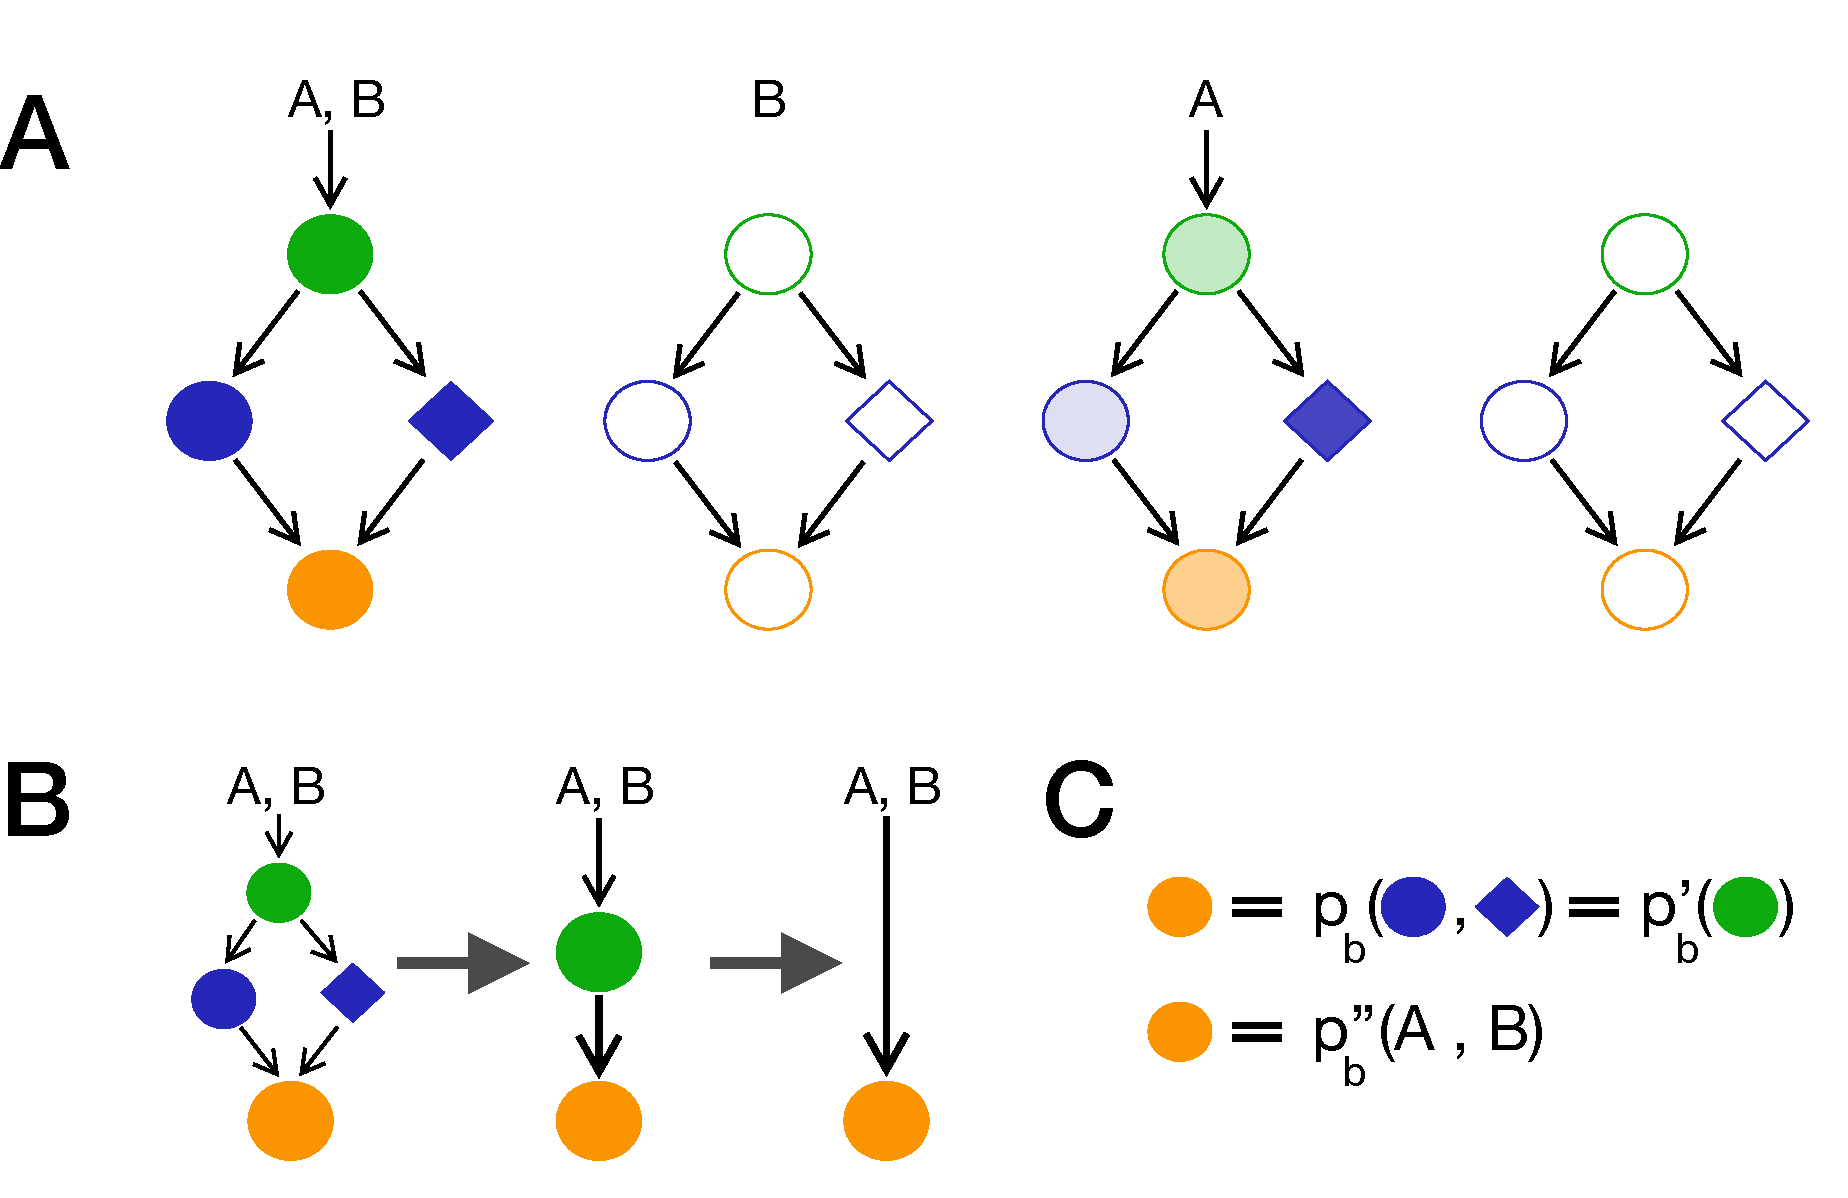
\includegraphics[width=\linewidth]{theoryims/Branching_Abbreviation.pdf}
  \caption{Signaling pathways can be abbreviated in genetic pathway
           representations.
           \textbf{A}. Two genes, \gene{a} and \gene{b},
           encoding protein products A and B respectively, interact to drive
           expression of a green gene, which in turn drives expression of two
           blue genes (through potentially distinct mechanisms). The blue genes
           then interact to drive expression of an orange gene. \gene{a} is
           epistatic over \gene{b}. Removing \gene{a} sends the green node to a
           a specific expression state. This state drives the blue genes into
           a specific state as well; then the blue genes drive the orange gene
           into a well-defined state. Removing \gene{b} sends the network into a
           completely different state. Since \gene{a} is epistatic over
           \gene{b}, mutating both genes sends the network into the same state
           as mutating \gene{a} alone.
           \textbf{B}. Since the network can only exist in three states (a
           wild type state, an \(a^-\) state and a \(b^-\) state), the network
           can be abbreviated to reflect that the state of the orange node can
           be completely specified by knowing the state (present or missing) of
           the upstream factors, \gene{a} and \gene{b}. \textbf{C}. This
           corresponds to stating that the probability that the orange node is
           transcribed can be expressed solely in terms of the protein products
           A and B when the products are expressed at wild-type levels or when
           one or the other product is completely missing.
           }\label{fig:branch}
\end{figure}

Another important question is whether there is an `optimal' choice of expression
phenotype. In other words, for a given graph containing nodes (genes) that can
interact (arrows) with other nodes, is there a `best' node to select as a
readout of the pathway (see Fig.~\ref{fig:branch})? For simplicity, but without
loss of generality, we envision a graph where a single, primary node accepts as
an input our two factors \(A\) and \(B\). This node can in turn drive expression of
a second layer of genes through arbitrary activation functions, and this second
layer can drive expression of a third layer of (completely different) genes.
Genes in this second layer are allowed to have any arbitrary interaction with
other genes in the second layer to drive expression of genes in the third layer.
This layering can repeat arbitrarily. We seek to answer the question: For an
arbitrary, acyclical graph, is there an `optimal' node that will reveal the
epistatic interactions between the two genetic factors \gene{a} and \gene{b},
assuming perfect measurements and zero biological noise?

Let us represent the expression level of the \(j\)th node in the \(i\)th layer
as \(p_{b, ij}\) following our previous notation. Clearly, the expression of the
primary node, \(p_{b, 00}\) depends on \(A\) and \(B\). We can write the
dependence of the state on these factors explicitly: \(p_{b, 00}(A, B)\). Then,
it follows that loss of \(A\) or \(B\) will send the state of this node to the
specific states, \(p_{b, 00}(0, B)\) and \(p_{b, 00}(A, 0)\) respectively. Since
\gene{a} is epistatic over \gene{b}, and \(A\) and \(B\) interact to drive this
node directly, then it follows that \(p_{b, 00}(0, B) = p_{b, 00}(0, 0)\). The
value \(p_{b, 00}(0, B)\) is an important quantity, therefore we assign it the
name \(P_{00}\). This proves node 00 can function as a suitable phenotype for
genetic analysis (by definition).

The second set of nodes \(p_{b, 1j}\) are regulated directly by node 00. We take
the activity of node 00 to be directly proportional to \(p_{b, 00}(A, B)\). Thus,
for any node 1\(j\), we can represent its expression level as
\(p_{b, 1j}(T[p_{b, 00}(A, B)])\), where \(T[\cdot]\) represents an arbitrary
time-independent function that transforms the expression level of 00,
\(p_{b, 00}\), into its product activity. Deletion of \gene{a} or \gene{b}
transmits directly into the expression states \(p_{b, 1j}(T[P_{00}])\) and
\(p_{b, 1j}(T[p_{b, 00}(A, 0)])\) respectively. Deleting \gene{a} and \gene{b}
simultaneously will cause the any node in layer 1 to enter the state
\(p_{b, 1j}(T[P_{00}])\). Since \(T[\cdot]\) is a time-independent function, it
follows that any node in layer 1 can be used as a gene expression phenotype,
regardless of any well-defined, non-trivial dependence it may have on node 00.
We can iterate this logic throughout any arbitrary number of layers. A layer can
drive expression of the next layer in any way without altering the ability of
the next set of nodes to function as indicators of the epistasis relationship
between \gene{a} and \gene{b}.

Taken together, these results explain why genetic diagrams need not represent
all factors between a pathway, and why genetic pathways are broadly insensitive
to spatial or temporal separation between components: Biological and
experimental noise would be the only limitations to detecting epistasis deep
into a directed acyclic graph. These results also highlight the fact that the
\emph{genetic diagrams} that emerge from time-independent epistatic analysis are
not necessarily informative about the dynamical behaviors of the \emph{molecular
interactions} that they result from because our genetic diagrams are constructed
in a digital fashion (presence or absence of a factor) and the phenotypes do not
contain temporal information that could inform us about these dynamics.

% \section*{The epistasis coefficient}
% \citet{Angeles-Albores2018a} introduced the notion of an epistasis coefficient.
% Briefly, the epistasis coefficient for gene expression measurements is defined
% as:
%
% \begin{equation}
%     s(a, b) = \frac{\log{FC_{ab} - \log{FC_a} - \log{FC_b}}}
%                     { \log{FC_a} + \log{FC_b}}.
% \label{eq:coeff}
% \end{equation}
% Here, $s(a, b)\) is the epistasis coefficient between \gene{a} and \gene{b};
% $FC_{x}\) is the fold-change in expression in mutants of genotype $x$ with
% respect to the wild-type; and $\log$ refers to the natural logarithm.
% Equation~\ref{eq:coeff} takes this form because we specified the null hypothesis
% of interaction to be log-additive. As a result, we can rewrite this equation
% in terms of observations and expectations:
%
% \begin{equation}
%     s(a, b) = \frac{\mathrm{Observed} - \mathrm{Expected}}{\mathrm{Expected}}.
% \end{equation}
%
% The epistasis coefficient can also be re-expressed using the language of
% statistical mechanics, if we define the fold-change to be the ratio of
% \(p_{bound}\) in the mutant relative to \(p_{bound}\) in the wild-type:
% $FC_x = p_{bound}^{mt}/p_{bound}^{wt}\). Performing
% this substitution allows us to inspect the values that $s(a, b)\) can take if \(A\)
% is epistatic to \(B\); that is to say, if Eq.~\ref{eq:epistasis} holds. Since
% Eq.~\ref{eq:epistasis}  is an identity, we can substitute $\log{FC_{ab}}\) with
% $\log{FC_{a}}\) in Eq.~\ref{eq:coeff}. Thus, when \gene{a} is epistatic to
% \gene{b}, Eq.~\ref{eq:coeff} simplifies to:
%
% \begin{equation}
%     s(a, b) = -\frac{\log{FC_b}}{\log{FC_a} + \log{FC_b}}.
% \end{equation}
%
% With this simplified form, we can ask what will happen as $FC_a$ changes.
% Consider the case where $FC_a = 1$, which means the epistasis coefficient is -1.
% This reflects the case where \gene{b} is a strong inhibitor of the gene activity
% of \gene{a}, such that $\gene{a}\) is not active in the experimental conditions
% (removing \gene{a} had no effect on gene expression). If $FC_a = FC_b$, this
% reflects a linear pathway, where \(A\) and \(B\) are both necessary for function in
% the pathway under study; this will correspond to an epistasis value of negative
% one half, $s(a, b) = -0.5$. If $\log{FC_a} < \log{FC_b}\), and the signs of
% $\log{FC_a}\) and $\log{FC_b}\) are the same, then the epistasis coefficient will
% have a value between $-1$ and $-0.5 $. On the other hand, if $\log{FC_a} >
% \log{FC_b}\) and both have the same sign, then the epistasis coefficient will lie
% between $-0.5$ and 0. These two cases correspond to branched pathways, where
% \gene{a} affects the transcriptional output via at least two different pathways,
% only some of which depend on \gene{b}. One notable characteristic of the
% epistasis coefficient is that for linear pathways, regardless of whether they
% are activating or inhibiting, the epistasis coefficient is guaranteed to be the
% same for all transcriptional elements downstream of the two genes under study.
%
% The epistasis coefficient, while a useful summary statistic, is not immune to
% pathologies. For example, if \gene{a} and \gene{b} have inverse effects on
% gene expression, such that $FC_a = FC_b^{-1}\), then the epistasis coefficient
% will become undefined. If Eq.\ref{eq:epistasis} holds, then we can still say
% that \gene{a} is epistatic over \gene{b}, but we should be wary of drawing a
% genetic pathway to explain this behavior, since we need more information. These
% examples help illustrate how the epistasis coefficient should be used. To
% perform an epistatic analysis using a transcriptional reporter, confirmation
% that Eq.\ref{eq:epistasis} holds is vital. Having confirmed that this identity
% applies, the epistasis coefficient can be computed to gain information into
% the nature of the interaction between the two genes in question (activating or
% inhibiting; linear or branched).

\subsection*{The requirements for epistatic analysis from a statistical
             mechanical perspective}
\subsubsection*{Null alleles.}
Geneticists have known for a long time that epistatic analyses must be carried
out using verified null alleles (alleles that do not generate product, or which
product is devoid of all biochemical activity). The reason for this requirement
becomes abundantly clear from Eq.~\ref{eq:epistasis2}. Since the genetic
activity of \gene{a} is modulated by \gene{b}, failure to use a null allele of
\gene{a} means that the loss of the activity provided by \gene{b} in the double
mutant will result in a measurable decrease of the activity of the gene product,
\(A\). Thus, the \Freg{} factor in the double mutant will not be the same as the
\Freg{} factor in the mutant of \gene{a}, and the equality requirement for
epistasis will be violated. Notably, a null allele of \gene{b} is not essential,
strictly speaking, to detect epistasis. However, failure to obtain a null allele
of \gene{b} will inhibit our ability to test whether the pathway via which these
genes interact is branched or not (see below).

\subsubsection*{Sensitization.}
Another difficulty with genetic analysis of a pathway can occur if the genes
under study are not major determinants of the phenotypic outcome. This is
equivalent to stating that \Freg{} depends on \(A\), \(B\) and at least one
other factor, \(C\); and that \(p_{bound}(A, B, C) \sim p_{bound}(0, 0, C)\).
The only case when Eq.~\ref{eq:pbound} suggests this can happen (in the absence
of measurement error) is when the effective polymerase activity, \(\rho\cdot
F_{reg}(0, 0, C)\) is very large. To study the functions of \gene{a} and
\gene{b} productively, it is necessary to re-scale \Freg{} to an appropriate
dynamic range such that \(p_{bound}\) is elastic to changes in the gene
activities of \gene{a} and \gene{b}. Since \Freg{} depends on the gene
activity of \gene{c}, the correct approach is to use an allele of \gene{c} that
decreases \Freg{} towards the desired direction. It is imperative that a
null allele of \gene{c} \textbf{not} be used, since \gene{c} may be epistatic to
\gene{a}, \gene{b} or both, in which case we would be unable to study
interactions between \gene{a} and \gene{b} in this genetic background. An
alternative to this strategy would be to decrease \(\rho\), but since RNA
polymerase is a crucial component of all cells, this is not advisable.

\subsection*{Genetic pathways in statistical mechanics}

\begin{figure}
  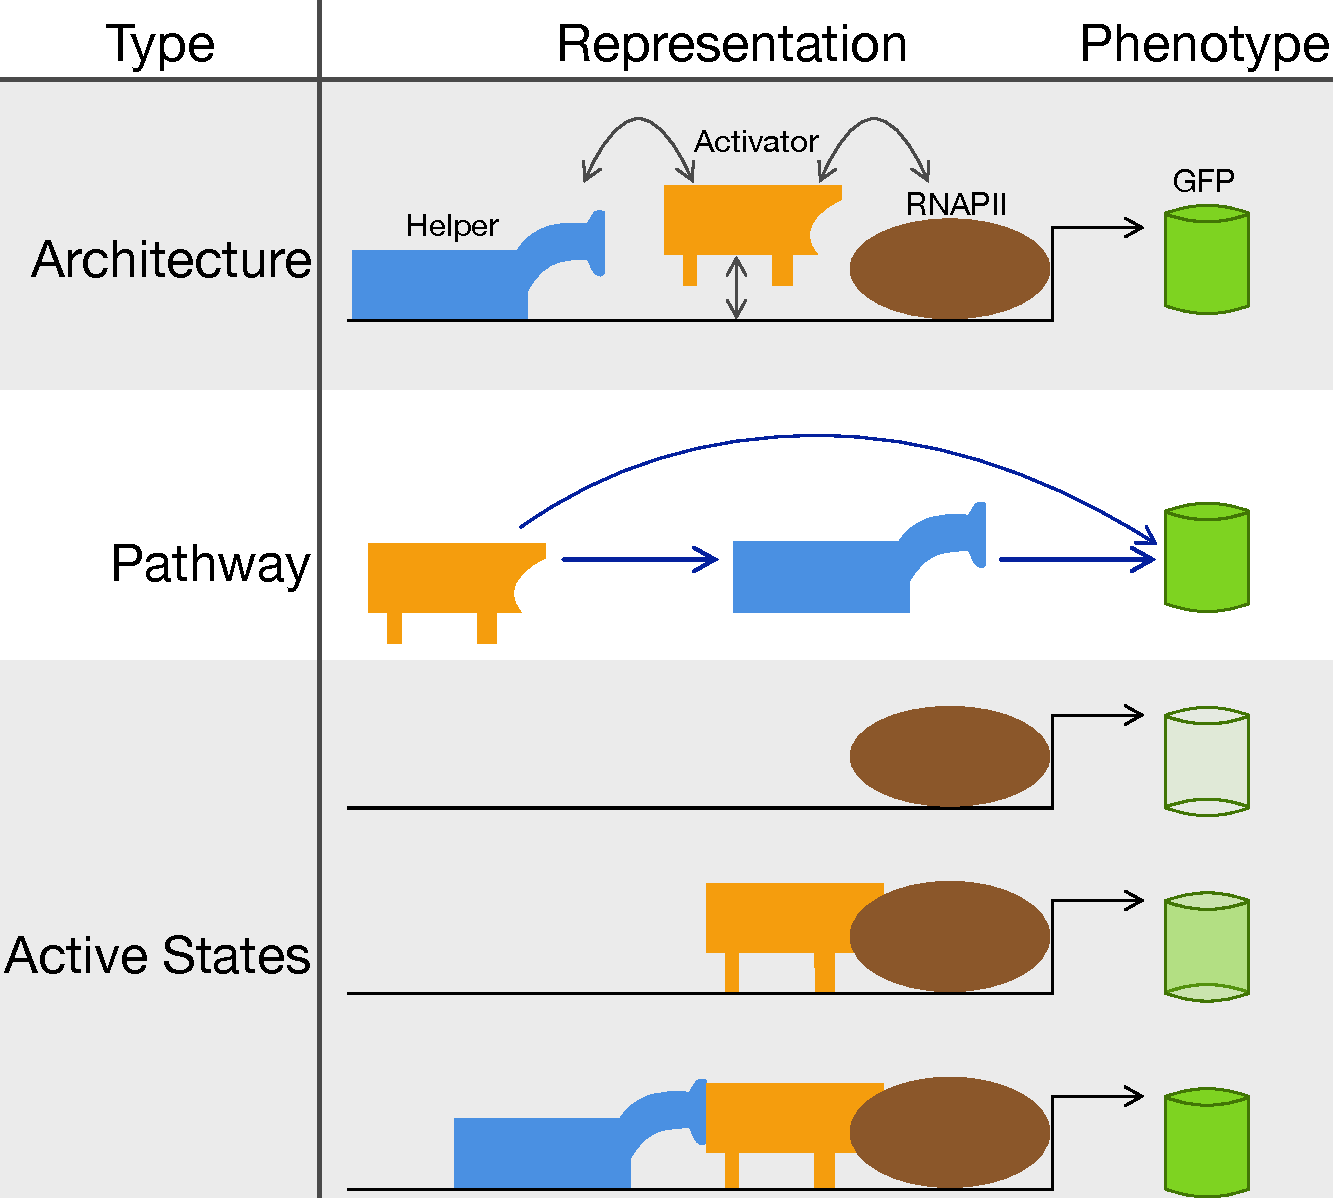
\includegraphics[width=\linewidth]{theoryims/Z_to_Genetics.pdf}
  \caption{Promoter architectures can be represented in three different ways.
  A promoter architecture can be represented by showing all the interactions
  between components simultaneously. An alternative representation is via
  genetic diagrams. The genetic diagram obviates the epistatic element. Finally,
  the statistical mechanical view is an enumeration of all the possible states
  in the promoter. In the above figure, only the active states are shown for
  brevity. A state is considered active if RNAPII is bound to the promoter.
  }\label{fig:Z_to_Genetics}
\end{figure}

Genetic diagrams are representations that satisfy observed epistasis
relationships between genes. Since we have found a mapping between epistasis
relationships and statistical mechanics, we can find the genetic pathway
equivalent to the states oriented picture of promoter architectures from
statistical mechanics (see Fig.~\ref{fig:Z_to_Genetics}). As a representative
example, envision a promoter architecture where there is an activator, \(A\),
which recruits RNA polymerase to the promoter and which can bind DNA with a
specific affinity; a helper or tethering protein, \(H\), that can bind the
activator as well as DNA, but cannot bind RNA polymerase; and RNA polymerase
present at some concentration. In this system, the helper molecule is not
necessary for activator function. The \Freg{} function for this system takes
the following analytical form:

\begin{equation}
    F_{reg}(A, H) = \frac{1 + A e^{-\varepsilon _{AP}}\frac{1 + H e^{-\varepsilon _{AH}}}
                                                       {1 + H}
                          }
                          {1 + A\frac{1 + H e^{-\varepsilon _{AH}}}
                                     {1 + H} }.
\label{eq:AH}
\end{equation}
Here, \(A\) and \(H\) represent the amount of activator and helper; \(\varepsilon _{AH}\)
is the energy of binding of activator to helper; and \(\varepsilon _{AP}\) is the
energy of binding of activator to polymerase. For simplicity, energies are
expressed in units of \(k_B T\).

As a first step, we confirm that this function satisfies the nested function
requirement for epistasis. We could re-write the above equation into a nested
function as follows:

\begin{equation}
    F_{reg}(A\cdot G_{reg}(H)) = \frac{1 + A e^{-\varepsilon _{AP}} \cdot G_{reg}(H)}
                                 {1 + A\cdot G_{reg}(H)}.
\label{eq:AHsimp}
\end{equation}

The fact that we can write this nested function means that the activator gene
is epistatic over the helper gene. Next, we will order the mutants according to
the magnitude of their \Freg{} factor. Since this is a system of activators,
the wild-type \(F_{reg}(A, B)\) must be greater than the value in any of the
mutants. Since \gene{a} is epistatic over \gene{b}, we know that \Freg{} for
the single mutant of \gene{a} and the double mutant have to be the same.
We also know that \Freg{} always increases with increasing effective gene
activity of \gene{a}, \(A\cdot G_{reg}(H)\). Finally, from inspection of
Eq.~\ref{eq:AH}, \(G_{reg}(0) = 1\). Putting all of this together, we can order
the factors:

\begin{equation}
F_{reg}[0] \leq F_{reg}[A \cdot G_{reg}(0)] \leq F_{reg}[A \cdot G(H)].
\end{equation}

This means that the phenotype of the double mutant \genotype{ab} and
\genotype{a} are of equal severity, and show the greatest perturbation relative
to the wild-type, while the single mutant of \gene{h} has a phenotype
intermediate to the phenotype of mutants of \gene{a} and the wild-type control.
Since the epistasis coefficient depends only on the \Freg{} associated with
each mutant, it follows that if we study how flexible this hierarchy can be,
we can study how this hierarchy can be modified by tuning the parameters in
Eq.~\ref{eq:AH}, and how this in turn can affect the value of the epistasis
coefficient.

We would like to know when
\(F_{reg}(A\cdot G_{reg}(0)) \sim F_{reg}[A \cdot G(H)]\).  This is equivalent to
stating that loss of \gene{h} does not measurably affect gene expression. This
will happen in the limit of saturating gene activity of \gene{a}, which results
from the combination of protein copy number, DNA binding affinity, and affinity
for RNA polymerase.
% This limit corresponds to an epistasis coefficient of 0,
% since the fold-change measured in null mutants of \gene{h} will be equal to 1.
% In this limit,
An epistatic analysis will conclude that \gene{a} and \gene{h}
do not interact along this phenotype and would identify a single pathway,
involving the activator gene, \gene{a}.

Another relevant limit is \(F_{reg}(0) \sim F_{reg}(A\cdot G_{reg}(0))\). For this
to be true, two conditions must hold. First, the gene activity of \gene{a} must
be low. Either the protein product is present at very low copy number or the
DNA binding affinity of the product is very low by itself. Second, the gene
activity of \gene{h} must not be low: It must have a reasonable combination of
protein copy number, DNA binding affinity and binding affinity to the product of
\gene{a} such that its regulatory function, \(G_{reg}(H)\) has a value much
greater than unity. In this regime, the single mutants of \gene{a} and \gene{h},
as well as the double mutant, would have the same fold-change relative to the
wild-type.
% In this case, the epistasis coefficient achieves a value of $-0.5$,
% which corresponds to a linear pathway.
This reflects the fact that the only
complex making a measurable contribution to polymerase binding is the complex
where the activator is bound to the helper. In other words, these two genes act
within a single, unbranched pathway that involves both \gene{a} and \gene{h}.

In between these two regimes, epistasis indicates the existence of two pathways,
one of which involves both \gene{a} and \gene{h}, and one of which involves only
\gene{a}. These pathways reflect the importance of an activator-polymerase
complex that does not include the helper protein; genetically, this secondary
complex constitutes a secondary, helper-independent pathway. The relative
importance of each pathway will depend strongly on the wild-type dosage levels.
This shows that statistical mechanical microstates can be mapped to genetic
pathways involving multiple genes. This mapping is not guaranteed to be
one-to-one (the mappings will usually be many-to-one), nor is it guaranteed to
describe all the states available to the pathway.

Although at no point is the equality in Eq.~\ref{eq:epistasis} violated, the
interpretation of the epistasis relationship is highly dependent on gene dosage.
Epistasis relationships are not immutable with dosage, and a given relationship
may change from independent to additive to suppressive along a given dosage
curve. This highlights the importance of varying the reference gene activity
levels using partial loss-of-function alleles to establish that
Eq.~\ref{eq:epistasis} holds along an entire curve.

\subsection*{Genetic Morphs}
Genetics can generate alleles with vastly different properties. Our formalism
allows us to immediately derive the most commonly encountered allele classes
(see Supplementary Information Section XXX: Common allelic classes and their
statistical mechanical definitions). In the following text, we assume the gene
in question promotes transcription; for an inhibitor, the definitions are the
same except that the effects on active and inactive states are flipped. An
active state is a state that has RNA polymerase bound.

\begin{itemize}
  \item \emph{Hypomorph}. \textbf{Genetic definition}: an allele with reduced
  gene activity, either by reduced product copy number or decreased biochemical
  activity, causing a loss-of-function mutant phenotype. \textbf{Statistical
  mechanical definition}: an allele which decreases the relative proportion of
  active states compared with the wild type homozygote.
  \item \emph{Hypermorph}. \textbf{Genetic definition}: an allele with increased
  gene activity, either by increased copy number or improved biochemical
  activity, causing an increased-function mutant phenotype; the hypermorphic
  phenotype can be phenocopied by overexpression of the wild type allele.
  \textbf{Statistical mechanical definition}: an allele that increases the
  relative proportion of active states compared with the wild type homozygote.
  \item \emph{Neomorph}. \textbf{Genetic definition}: an allele which has a
  novel functionality causing a mutant phenotype which cannot be phenocopied
  simply by overexpressing wild type product. The neomorphic allele generates
  product at a similar rate as the wild type allele. \textbf{Statistical
  mechanical definition}: an allele encoding a modified \Freg{} function,
  generating novel states (active or inactive) not accessible to the wild type
  product at any concentration.
\end{itemize}

Grouping alleles into the correct change-of-function classes is an important
part of genetic analysis because hypermorphic alleles from one gene can be used
in combination with null alleles at a second locus to order genes in a pathway.
However, neomorphic and hypermorphic alleles can be extremely difficult to
discern and can confound genetic analysis. From a statistical mechanical
perspective, this confounding arises because the neomorphic allele
changes the functional form of the interactions, which qualitatively alters
the system by adding neofunctionalized states, whereas the hypermorphic allele
exclusively changes the gene dosage relative to the wild-type levels.

\section*{Discussion}
We have shown that genetics is a method to study partition
functions that are not known analytically. The method relies on systematically
setting component values to zero, individually and pairwise, and identifying
circumstances when the partition function exhibits epistasis. Although equality
between two sets of perturbations can occur as a coincidence, the stringent
requirement of equality makes this an unlikely occurrence. Therefore, if
there is epistasis between two components, it is reasonable to infer that these
perturbed variables function as a single variable equal to a product of two
functions that each take as input one of the two component. This methodology is
known in genetics as epistatic analysis, and it provides a way to study, in an
analog fashion, a molecular system where the components and interactions may be
entirely unknown.

The results from epistatic analyses can be represented as genetic diagrams,
where the genes represent a component in the system and arrows indicate
interactions. Because of the analog nature of the analysis (components are
either `ON' or `OFF'), genetic diagrams do not have to yield information about
the dynamical capacities of the system, nor do they represent direct biochemical
interactions. Rather, genetic pathways are a graphical method of representing
epistatic interactions between components in a circuit, allowing geneticists to
rapidly identify the epistatic and hypostatic components in any given
comparison, and the weighting given to different arrows depends strongly on the
dosage of all the components connected by them. When these pathways are drawn to
represent elements of a promoter, pathways can be mapped onto subsets of active
states involving the elements connected by arrows.

Gene expression levels are increasingly being used as a phenotype for genetic
analysis. A particularly attractive feature of these phenotypes is our ability
to measure expression levels in a highly multiplexed fashion in a single
experiment, but the resulting datasets have proven hard to analyze due to their
high-dimensional nature. Dimensionality reduction methods such as principal
component analysis or non-negative matrix factorization have become popular ways
to analyze transcriptomic data. However, a drawback of these methods is that
they are derived from a statistical framework without connection to the
underlying biology, and the transformations that they apply to the data make it
difficult to interpret signals in terms of biological components. Another
powerful approach is to fit general linear models with interactions terms to
transcriptomic dataset. In this framework, the expression level of an individual
transcript is modeled with two first order coefficients that quantify the
independent effect of each component on the expression level of that transcript,
and an interaction term that is non-zero when the double mutant shows
non-additive expression levels. Here, we argue that this approach does not
extract all the available information encoded in transcriptomes because it does
not, on its own, identify cases where classical epistasis is occurring.

We have shown that, for systems at equilibrium, epistasis arises naturally.
Moreover, we have shown that epistasis percolates through a network at
equilibrium regardless of its depth, and we speculate whether this result may
explain the unreasonable effectiveness of genetics at enormous differences in
scale, since macroscopic (organismal or population) phenotypes to microscopic
phenotypes all show epistasis. However, a major caveat to this work is the
fact that biological systems are not at thermal equilibrium. The commonality of
classical epistasis in biological systems suggests that many of our results will
have a non-equilibrium analog with some changes. Certainly, networks that are
not at equilibrium will not reveal epistasis at arbitrary depth. For
non-equilibrium networks, it will be particularly interesting to study how
epistasis is affected by relaxing the acyclic requirement we imposed. Feedback
might be expected to hide epistasis; however, biological experiments suggest
that certain topologies, even with feedback, show epistasis robustly. The study
of the physical basis of epistasis in biological systems seems poised to reveal
fascinating new insights into the principles of how these networks are built.
